\section*{Question 6:}
Extra Credit: SVMlight, 10 points extra credit:


see: http://www.cs.cornell.edu/People/tj/svm\_light/


* 1 point:


work through the "Inductive SVM" example, discuss in detail the steps and resulting output

\subsection*{Answer:}

I downloaded and installed the SVM light from: 

http://www.cs.cornell.edu/people/tj/svm\_light/

I followed the installation instructions and downloaded the Inductive SVM example.

I also followed the instructions to run svm\_learn and passed the training data file train.dat as a command line argument. It produced the model file, which I used as an input for the program svm\_classify.

I saved the entire session in the file svm.txt under Q6 folder. 

Below is the content of the file. 

\lstinputlisting[language=bash, breakatwhitespace=〈false), label=The content of svm.txt, caption= The content of svm.txt]{Q6/svm.txt}

The results were printed on the screen:

\begin{figure}[h]
\caption{Inductive SVM Example}
\centering
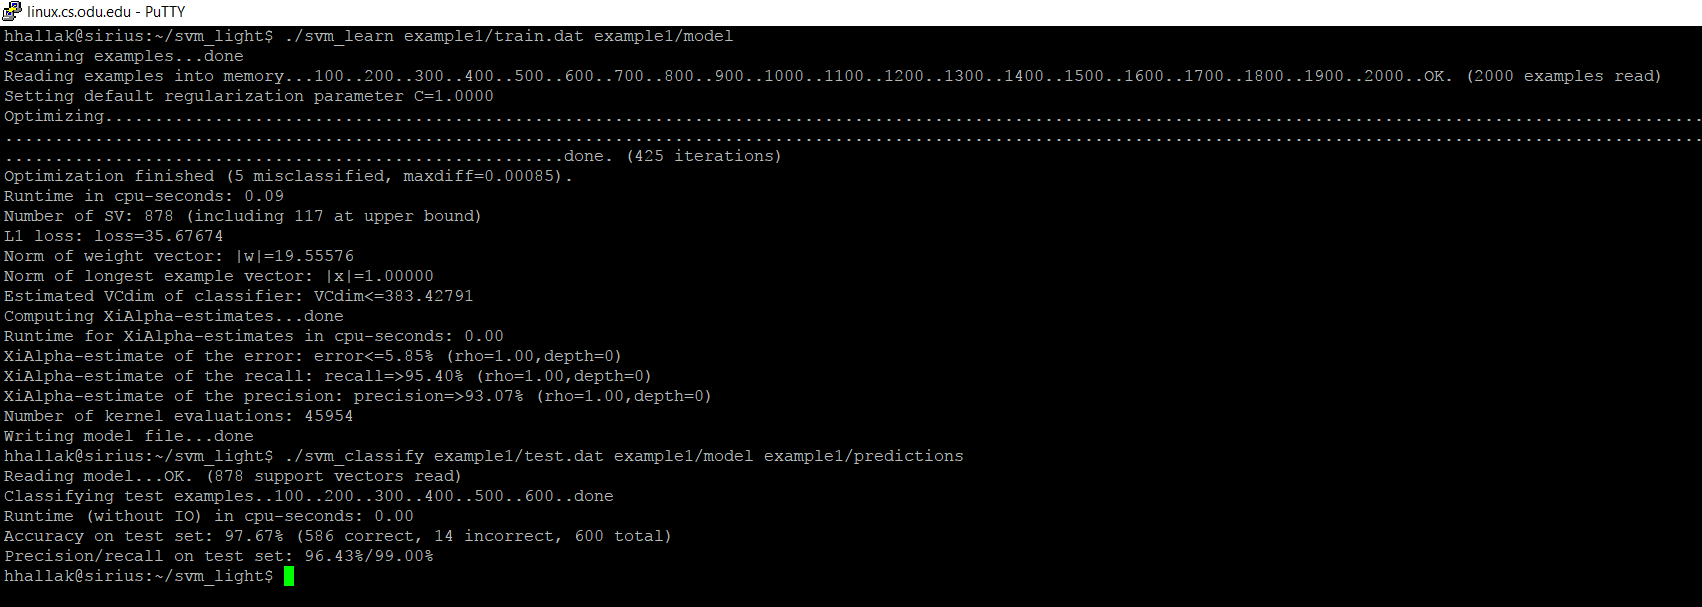
\includegraphics[scale=0.4]{Q6/svm.png}
\end{figure}

Accuracy on test set: 97.67% (586 correct, 14 incorrect, 600 total)

Precision/recall on test set: 96.43%/99.00%

The results show that these scores are very high for these measures.